\section{Dataset Preparation}\label{sec:preprocessing}
Sound data preprocessing is crucial for a generalizable model. In \Cref{sec:prep:existing}, the preprocessing approach from \citet{jiang_automatically_2017} is discussed. \Cref{sec:prep:new} proposes an alternative, more rigorous preprocessing technique. \Cref{sec:prep:analysis} discusses the characteristics of preprocessed datasets.

\subsection{Reference Method}\label{sec:prep:existing}
% In order to evaluate the performance of the model described in \Cref{subsec:model}, the exact dataset from

\citet{jiang_automatically_2017} use their own dataset containing 2M commits from the top 1000 Java projects on GitHub, published earlier in \cite{jiang_towards_2017}. Commit messages and diffs are cleaned and filtered, to arrive at a final dataset of 32k <commit,diff> pairs.

The dataset is filtered by removing merge and rollback commits and diffs larger than 1MB. Diffs containing more than 100 tokens and commit messages with more than 30 tokens are discarded. Then, a Verb-Direct Object filter is applied to commit messages and selects only messages starting with a verb that has a direct object dependant \cite{jiang_automatically_2017}. 

The commit messages are cleaned by extracting only the first sentence and removing issue IDs; diffs are cleaned by removing commit IDs. Both diffs and commit messages are tokenized by whitespace and punctuation \cite{jiang_automatically_2017}.

% We continue with preprocessing the collected commits, which consist of both the commit messages and the commit diffs. For the messages we take a similar approach as Jiang et al \cite{jiang_automatically_2017}. On top of the steps taken in their paper, we introduce multiple additional preprocessing steps.
% \\todo{Where in this process is filtered on .java .md and .txt files?}

% \todo{Explain vocab limitation elsewhere}

\subsection{Alternative Method}\label{sec:prep:new}
\citet{liu_neural-machine-translation-based_2018} thoroughly analyzed the dataset from \cite{jiang_automatically_2017} and found that their dataset is noisy. To improve the quality of the dataset -- the hypothesis is that more extensive preprocessing would enable a model to better learn and generalize over the relations between code changes and commit messages -- the preprocessing pipeline proposed by \cite{jiang_automatically_2017} is extended.

First, a preliminary filter is applied that removes all merge and rollback commits, which are unsuitable to be used for machine translation \cite{jiang_automatically_2017}. Then, commit messages and diffs are processed as follows.

\subsubsection{Commit Messages}

\begin{enumerate}
\item \textit{Cleaning.} GitHub issue IDs, preceding labels in the format "\textit{[Label]} Sentence.", \textit{@mentions}, URLs and SHA-1 (commit) hashes are removed from the commit messages. Furthermore, all version numbers are replaced with a placeholder token and sub-tokens (\underline{c}amel\underline{C}ase) are split. Lastly, based on \citet{liu_generating_2019}, non-English characters are removed and the commit message is lowercased.

\item \textit{Tokenizing.} Sentences is commit messages are first parsed with the NLTK Punkt sentence tokenize. Only the first sentence of the first line of a commit is retained. This sentence is then parsed by natural language toolkit SpaCy to extract tokens and their respective part-of-speech (PoS) tags. Redundant whitespace and trailing punctuation is removed.

\item \textit{Message Length Filter.} Commit messages with less than 2 or more than 30 tokens are removed.

\item \textit{Verb Filter.} Automated PoS-tagging is prone to errors if the source text uses invalid grammar. Initial experiments have shown that verbs are often classified as nouns, because developers write concise commit messages, omitting the subject of a sentence. The V-DO constraint is therefore relaxed by only requiring that a sentence starts with a verb. If the first word is not classified as verb at first, a secondary check on the message, prepended with "\textit{I}", is performed to select any remaining messages. An example construct is shown in \Cref{fig:verb_detection_error}.

\begin{figure}
    \centering
    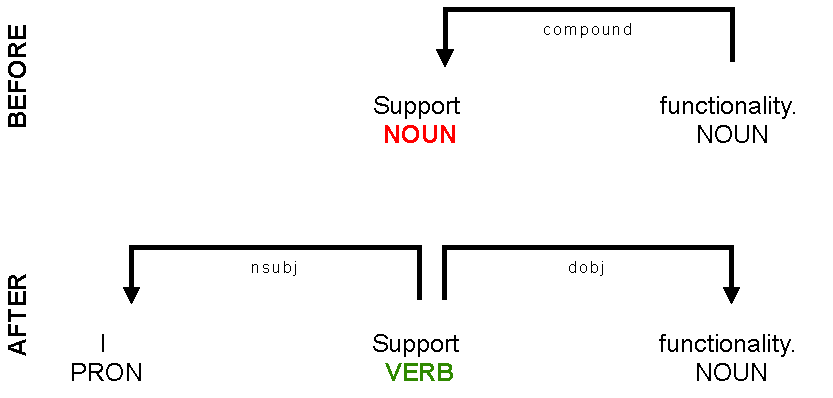
\includegraphics[width=.75\linewidth]{figs/verbs_wrong.pdf}
    \caption{Automated verb detecting correction by prepending pronoun.}
    \label{fig:verb_detection_error}
\end{figure}
\end{enumerate}

\subsubsection{Diffs}
Contrary to the approach of \citet{jiang_automatically_2017}, diffs are also subject to preprocessing. The hypothesis is that diffs contain a lot of redundant information that is not informative for commit message generation.

\begin{enumerate}
    \item \textit{Parsing.} Diffs are split into blocks per file, which are processed further independently. Only files with either additions or deletions are kept.
    
    \item \textit{Cleaning.} Instead of the full path to the changed file, only the filename and extension is retained. The location of the change is removed and only the context of the change (encapsulating method or class name) is kept. Again, sub-tokens are split, non-English tokens are removed and all tokens are lowercased.
    
    \item \textit{Filtering.} Diffs with more than 100 tokens are discarded. Only changed files with a whitelisted extension are kept, changed lines from other files are removed from the diffs. Finally, the files in the diff are sorted on by most lines changed.
    
    \item \textit{Tokenizing.} Diffs are tokenized on whitespace and punctuation. The tokenizer used is an improved version of the \textit{WordPunctTokenizer}\footnote{\url{https://www.nltk.org/api/nltk.tokenize.html\#module-nltk.tokenize.punkt}}, which does not split language operators or comment indicators (e.g. \texttt{++}, \texttt{//}, etc.)
\end{enumerate}

\subsection{Processed Dataset Characteristics}\label{sec:prep:analysis}
The novel preprocessing method is applied to both the dataset collected by \citet{jiang_towards_2017} and the Java and C\# datasets collected in this work. 

\subsubsection{Dataset Sizes}
\Cref{tbl:dataset_processing} contains an overview of the processed datasets. Substantially more commits are retained from the dataset collected by \citet{jiang_towards_2017} than originally. The reason for this is twofold: \citet{jiang_automatically_2017} only keep commits starting with one of the 20 most occurring verbs, instead of applying no such filter. This makes their dataset naturally smaller. Furthermore, they discard commit messages that start with a verbs that are not classified as such by their natural language processor, instead of making an effort to better detect verbs.

\begin{table}[]
\caption{Dataset sizes before and after processing.}
\label{tbl:dataset_processing}
\begin{tabular}{@{}lll@{}}
\toprule
\textbf{Dataset} & \textbf{Original} & \textbf{Processed} \\ \midrule
         Java Top 1000    & 610K & 151K \\
         C\# Top 1000     & 1.6M & 389K \\
         NMT1 \cite{jiang_automatically_2017} & 2.1M & 32K \\
         NMT1 (processed) & 2.1M & 156K \\
         \bottomrule
\end{tabular}
\end{table}

\subsubsection{Diff Length Distribution}\label{subsec:difflength}
\citet[fig.5]{jiang_automatically_2017} have analyzed the distribution of diff lengths in their test set and found that the distribution is heavily skewed towards the maximum number of 100 tokens. \Cref{app:vis:tokendist} (a) reproduces this distribution for the convenience of the reader. Additionally, the diff length distribution is visualized (\Cref{app:vis:tokendist} (b), (c) and (d)) for every processed dataset used in this work. The distribution is remarkably different: the long tail is gone and the diff lenghts are more or less evenly distributed. This phenomenon can be explained by the removal of entire file paths but the filenames from diffs, which decreases the expected minimum length for files changed in nested folders.
